\documentclass{scrreprt}
\usepackage{amsmath}
\usepackage{listings}
\usepackage{array}
\usepackage{tikz} 
\usepackage{underscore}
\usepackage[bookmarks=true]{hyperref}
\usepackage[utf8]{inputenc}
\usepackage[english]{babel}
\usepackage{enumitem}
\usepackage[a4paper, margin=1in]{geometry}
\usetikzlibrary{shapes, arrows.meta, positioning, backgrounds}
\usetikzlibrary{arrows.meta}
\usetikzlibrary{shapes.geometric, positioning, arrows.meta}
\usetikzlibrary{positioning}
% Define styles for different node types
\tikzstyle{startstop} = [rectangle, rounded corners, minimum width=3cm, minimum height=1cm, text centered, draw=black, fill=red!30]
\tikzstyle{process} = [rectangle, minimum width=3.5cm, minimum height=1cm, text centered, draw=black, fill=blue!30]
\tikzstyle{arrow} = [thick,->,>=stealth]
% Define stickman style
\tikzset{
    startstop/.style={
        rectangle, rounded corners, minimum width=3cm, minimum height=1cm, text centered, draw=black, fill=gray!30
    },
    process/.style={
        rectangle, minimum width=3cm, minimum height=1cm, text centered, draw=black, fill=blue!30
    },
    decision/.style={
        diamond, aspect=2, minimum width=3cm, minimum height=1cm, text centered, draw=black, fill=orange!30
    },
    arrow/.style={
        thick, ->, >=stealth
    },
    stickman/.pic={
        % Head
        \draw[fill=gray] (0,0.6) circle (0.3cm);
        % Body
        \draw[line width=0.5mm] (0,0.3) -- (0,-0.6);
        % Arms
        \draw[line width=0.5mm] (-0.4,0.3) -- (0.4,0.3);
        % Legs
        \draw[line width=0.5mm] (0,-0.6) -- (-0.4,-1.2);
        \draw[line width=0.5mm] (0,-0.6) -- (0.4,-1.2);
}
}
\hypersetup{
    bookmarks=false,    % show bookmarks bar?
    pdftitle={Software Requirement Specification},    % title
    pdfauthor={Jean-Philippe Eisenbarth},                     % author
    pdfsubject={TeX and LaTeX},                        % subject of the document
    pdfkeywords={TeX, LaTeX, graphics, images}, % list of keywords
    colorlinks=true,       % false: boxed links; true: colored links
    linkcolor=blue,       % color of internal links
    citecolor=black,       % color of links to bibliography
    filecolor=black,        % color of file links
    urlcolor=purple,        % color of external links
    linktoc=page            % only page is linked
}
\usetikzlibrary{shapes, arrows.meta, positioning, backgrounds}

\tikzstyle{startstop} = [rectangle, rounded corners, minimum width=3cm, minimum height=1cm, text centered, draw=black, fill=red!30]
\tikzstyle{process} = [rectangle, minimum width=3.5cm, minimum height=1cm, text centered, draw=black, fill=blue!10]
\tikzstyle{database} = [rectangle, minimum width=3cm, minimum height=1cm, text centered, draw=black, fill=orange!30]
\tikzstyle{auth} = [rectangle, minimum width=3cm, minimum height=1cm, text centered, draw=black, fill=green!30]
\tikzstyle{ui} = [rectangle, minimum width=3.5cm, minimum height=1cm, text centered, draw=black, fill=yellow!30]
\tikzstyle{arrow} = [thick,->,>=stealth]



\usepackage{hyperref}
% Set extra row height and padding
\setlength{\extrarowheight}{4pt} % Adds extra height between rows
\renewcommand{\arraystretch}{1.5} % Increases the height of each row

\begin{document}
\begin{titlepage}
    \centering
    \begin{center}
        
\includegraphics[width=0.5\textwidth]{logo.png} % Adjust width as necessary
    \end{center}
\begin{center}
    \textbf{Department of Computer Science and Engineering}\\
    Premier University
\end{center}
\begin{center}
    \huge \textnormal{CSE 305: Software Engineering \& Information System 
                     Design}
    \vspace{1in} % Adjusts vertical space after the course title
    \newline
    \Large \textnormal{Title: CT-03 Assignment}
    \vspace{0.5in} % Adjusts vertical space after the assignment title
\end{center}

    \large
    \textbf {Submitted by}\\
   \begin{center}
\renewcommand{\arraystretch}{1.5} % Adjusts vertical spacing in the table
\begin{tabular}{|p{0.4\textwidth}|p{0.6\textwidth}|} % Set column widths to 20% and 80%
\hline
\textbf{Name} & Mohammad Hafizur Rahman Sakib \\
\hline
\textbf{ID} & 0222210005101118 \\
\hline
\textbf{Section} & C \\
\hline
\textbf{Session} & Spring 2024 \\
\hline
\textbf{Submission Date} & 10.09.2024 \\
\hline
\end{tabular}
\end{center}

    \vspace{0.5in}
 
\begin{minipage}[t]{0.5\textwidth}
        \textbf{Submitted to :}
        \\Jannatul Maowa Hasi
        \\Lecturer,Department of CSE
        \\ Premier University
        \\ Chittagong
    \end{minipage}%
    \begin{minipage}[t]{0.6\textwidth}
        \raggedleft
        \textbf{Remarks}\\
        \vspace{0.5cm} % Adjust vertical space for remarks
        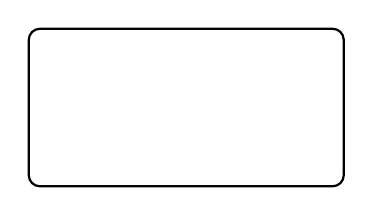
\begin{tikzpicture}
            \draw[thick, rounded corners] (0,0) rectangle (4,2);
        \end{tikzpicture}
    \end{minipage}

    \date{\today}
    \vfill
\end{titlepage}

\section*{Cost Analysis}

\begin{table}[h!]
\centering
\begin{tabular}{|p{8cm}|p{4cm}|}
\hline
\textbf{Cost Category} & \textbf{Amount} \\
\hline
\textbf{Initial Investment} & \\
\hline
\hspace{10pt} Software License & \$50{,}000 \\
\hline
\hspace{10pt} Hardware Upgrades & \$10{,}000 \\
\hline
\hspace{10pt} Implementation Costs & \$20{,}000 \\
\hline
\hspace{10pt} Training Costs & \$5{,}000 \\
\hline
\hspace{10pt} Utilities Cost (Yearly) & \$1{,}500 \times 12 = \$18{,}000 \\
\hline
\textbf{Marketing Costs} & \$40{,}000 (Approximately) \\
\hline
\textbf{Other Costs} & \\
\hline
\hspace{10pt} Maintenance and Support (Yearly) & \$10{,}000 \\
\hline
\hspace{10pt} Data Storage (Yearly) & \$2{,}000 \\
\hline
\textbf{Total Development Cost} & \textbf{\$155{,}000} \\
\hline
\end{tabular}
\caption{Cost Analysis}
\end{table}

\section*{Benefit Analysis}

\subsection*{1. Increased Sales}
A 10\% increase in annual revenue:
\[
\text{Present revenue} = \$1{,}000{,}000
\]
\[
\text{Increase} = 0.10 \times 1{,}000{,}000 = 100{,}000
\]

\subsection*{2. Customer Satisfaction}
50\% of new customers become regular customers:
\[
\text{New customers contributing} = 0.50 \times \text{new customers} \times 5000
\]

\subsection*{3. Reduced Labor Costs}
Replacing 3 workers, each paid \$30/hour:
Assuming 40 hours/week, 52 weeks/year:
\[
\text{Savings per worker} = 30 \times 40 \times 52 = 62{,}400
\]
\[
\text{Total Savings} = 62{,}400 \times 3 = 187{,}200
\]

\subsection*{4. Increased Brand Value}
Assuming a 25\% increase in brand value will contribute additional revenue. This is difficult to quantify exactly but may contribute to customer loyalty and new customer acquisition.

\subsection*{5. Adjust for Dollar Rate Decrease}
Each year, the value of the dollar decreases by 15\%. This affects both costs and benefits, but we'll assume it's more relevant to the recurring costs.

\section*{Payback Period Calculation}

\begin{table}[h!]
\centering
\begin{tabular}{|p{6cm}|p{2cm}|p{2cm}|p{2cm}|p{2cm}|p{2cm}|p{2cm}|}
\hline
\textbf{Cash Flow Description} & \textbf{Year 0} & \textbf{Year 1} & \textbf{Year 2} & \textbf{Year 3} & \textbf{Year 4} & \textbf{Year 5} \\
\hline
\textbf{Cost} & \$155{,}000 & \$12{,}000 & \$12{,}000 & \$12{,}000 & \$12{,}000 & \$12{,}000 \\
\hline
\textbf{Benefit} & \$0 & \$780{,}000 & \$780{,}000 & \$780{,}000 & \$780{,}000 & \$780{,}000 \\
\hline
\textbf{Net Cash Flow} & (\$155{,}000) & \$768{,}000 & \$768{,}000 & \$768{,}000 & \$768{,}000 & \$768{,}000 \\
\hline
\textbf{Cumulative Cash Flow} & (\$155{,}000) & \$613{,}000 & \$1{,}381{,}000 & \$2{,}149{,}000 & \$2{,}917{,}000 & \$3{,}685{,}000 \\
\hline
\end{tabular}
\caption{Payback Period Calculation}
\end{table}

\section*{Payback Period Determination}

The cumulative cash flow becomes positive after the first year, therefore the payback period is:

\textbf{Payback Period: 1 Year}

\section*{ROI Analysis}

The ROI (Return on Investment) can be calculated using the following formula:

\[
\text{ROI} = \frac{\text{Total Benefits} - \text{Total Costs}}{\text{Total Costs}} \times 100
\]

\begin{align*}
\text{Total Costs} &= \$155{,}000 \text{ (Initial)} + \$12{,}000 \text{ (Ongoing Year 1)} \\
&= \$167{,}000 \\
\text{Total Benefits (Year 1)} &= \$780{,}000 \\
\text{ROI} &= \frac{780{,}000 - 167{,}000}{167{,}000} \times 100 \approx 466.47\%
\end{align*}

\textbf{ROI for Year 1: 466.47\% and Payback Period: 1 Year}
\newline

This analysis shows that the investment in the software system will be fully recovered within 1 year, with a high ROI of 466.47\% by the end of the first year.

\end{document}
